\documentclass[11pt]{article}
\usepackage{amsmath, amssymb}
\usepackage{hyperref}
\usepackage{graphicx}
\usepackage{tikz}

\newcommand{\problemname}[1]{\section*{#1}}
\newcommand{\illustration}[3]{%
    \begin{figure}[h]
        \centering
        \includegraphics[width=#1\textwidth]{#2}
        \caption{#3}
    \end{figure}
}
\begin{document}
\problemname{The Evil Letter}
You are writing a very important essay for a notoriously strict professor. Unfortunately, your professor believes that some characters carry ``evil energy'' and wants you to avoid using them too much.

To measure how \emph{evil} a character is, the professor uses its \textbf{ASCII value}. A character with a higher ASCII value is considered more evil. For example, the characters \texttt{a}, \texttt{x}, and \texttt{)} have ASCII values $97$, $120$, and $41$ respectively, so \texttt{x} is the most evil among them.

Your essay is given as a string of characters. The professor defines the \emph{$k$-th most evil character} as the character whose ASCII value is the $k$-th largest among all characters in the essay (counting duplicates separately). Your task is to identify this character.

\begin{figure}[h]
\centering
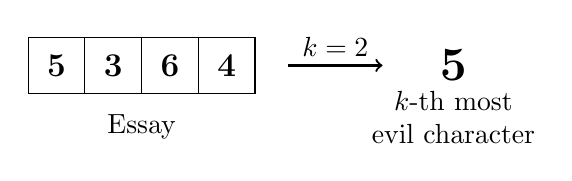
\begin{tikzpicture}[scale=0.6]
    % array boxes
    \foreach \x/\val in {0/5, 1/3, 2/6, 3/4} {
        \draw (\x*1.2, 0) rectangle +(1.2, 1.2);
        \node at (\x*1.2 + 0.6, 0.6) {\large \textbf{\val}};
    }
    

    \node at (2.4, -0.7) {Essay};
    
    \draw[->, thick] (5.5, 0.6) -- (7.5, 0.6);
    \node at (6.5, 1.0) {$k=2$};
    
    \node at (9, 0.6) {\LARGE \textbf{5}};
    
    \node[align=center] at (9, -0.5) {$k$-th most \\ evil character};
    
\end{tikzpicture}
\caption{\footnotesize Visualization of the $k$-th most evil character concept using sample input}
\label{fig:kth-evil}
\end{figure}

However, there is a catch: the professor has a terrible memory and uses an old writing tool that cannot store the whole essay in extra memory. You are only allowed to keep track of a small number of candidate characters at any time, instead of sorting or copying the entire essay in a separate data structure.

Formally, let $s$ be a string of length $n$. For each character $c$ in $s$, define
\[
f(c) = \text{ASCII value of } c.
\]
Consider the multiset
\[
\{f(s_1), f(s_2), \ldots, f(s_n)\}.
\]
If we sort these values in non-increasing order (from largest to smallest), the $k$-th value in this order corresponds to the $k$-th most evil character. You must output \emph{that} character.

Note that if the same character appears multiple times, each occurrence is counted separately. For example, if $s = $ \texttt{xxa} and $k = 2$, then the ASCII values are
\[
\{120, 120, 97\}
\]
and both the first and second most evil characters are \texttt{x}.

Because of the professor's memory limitations, your solution should use only a small amount of extra space besides the input itself (e.g., keeping track of only $O(k)$ candidate characters at any time).

\section*{Input}
The input consists of two lines:
\begin{itemize}
\item The first line contains two integers $n$ and $k$ ($1 \le k \le n \le 200\,000$), the length of the essay and the desired rank of evilness.
\item The second line contains a string $s$ of length $n$. Each character of $s$ is a visible ASCII character in the range $33$ to $126$ (from \texttt{!} to \texttt{\textasciitilde}). There are no spaces in $s$.
\end{itemize}

\section*{Output}
Output a single character: the $k$-th most evil character in the essay, i.e., the character whose ASCII value is the $k$-th largest among all characters in $s$ (counting duplicates separately).

\begin{tabular}{|l|l|}
\hline
{\footnotesize\textbf{Sample Input 1}} & {\footnotesize\textbf{Sample Output 1}} \\
\hline
\begin{minipage}[t]{0.45\textwidth}
\vspace{0pt}
\ttfamily
4 2\\
5364
\end{minipage}
&
\begin{minipage}[t]{0.45\textwidth}
\vspace{0pt}
\ttfamily
5
\end{minipage}
\\
\hline
\end{tabular}

\vspace{1em}

\begin{tabular}{|l|l|}
\hline
{\footnotesize\textbf{Sample Input 2}} & {\footnotesize\textbf{Sample Output 2}} \\
\hline
\begin{minipage}[t]{0.45\textwidth}
\vspace{0pt}
\ttfamily
3 1\\
ax)
\end{minipage}
&
\begin{minipage}[t]{0.45\textwidth}
\vspace{0pt}
\ttfamily
x
\end{minipage}
\\
\hline
\end{tabular}

\end{document}
